\label{sec:intro}

% single applicaiotn -> performance + power


%The hardware nodes of a cloud service provider are often each dedicated to running a single cloud service component~\cite{FB}.
As latency-critical tasks become ubiquitous across data centers,
deploying them on dedicated nodes is becoming a well studied and favored decision~\cite{ixcp, heracles, PerAppPower, twine}.
Typically, this dedication prevents latency violations that might be triggered
by the co-location of best-effort batch tasks.
One hopes that this dedicated nature (i.e. fixed role in the service using a fixed software stack) can be exploited to obtain the required performance (e.g. 99\% tail latency) while minimizing the energy used, a key concern given the increasingly constrained energy budgets in data centers~\cite{ixcp, SmoothOperator, Dynamo, oldi-study, oldi-pegasus, NLP-energy}.

%General purpose OSes such as Linux have been designed to support a range of user software as well as the concurrent execution of competing applications, thus, they have evolved to include support for dynamically adjusting various hardware settings on modern CPUs and network interface cards (NICs). Past researchers have demonstrated that dedicating a node to a single application can attain dramatic performance gains~\cite{ix,arrakis, exokernel,ebbrt,rumpkernel, unikernels, aliraza}, these results also suggest that one may be able to cater a node's hardware parameters to obtain higher efficiency than allowing the OS to dynamically adjust them.

%While researchers have proposed application specific OSes in the past, their optimizations have mainly focused on OS level changes targeting performance.

%However, dedicating a node to a single application suggests that one may be able to manually tune the node's hardware settings to magnifiy the impact of such tuning. While researchers have proposed such systems in the past, referred to as library OSes~\cite{ix,arrakis, exokernel,ebbrt} or unikernels~\cite{rumpkernel, unikernels, aliraza}, this 
%Dedicating a node to a single application suggests that one may be able to manually tune the node's hardware parameters to fixed values and obtain higher efficiency than allowing the OS to dynamically adjust them.  Furthermore, it is possible that the impact of hardware tuning can be magnified if one starts with an application specific OS that has been designed and implemented for running a single dedicated application. 

However, the performance and energy use of a system are complex emergent properties of the myriad of interactions between application software, operating systems, hardware, and offered loads.
Interestingly, when we take a careful look at overall system execution under different energy profiles, we see that the consequences of tuning energy and performance reach far beyond directly observable quantities and impact the interactions between the aforementioned system components in subtle ways.
There is a dizzying array of operating system mechanisms and policies one must consider that could both individually and collaboratively impact the performance and energy use of the system.
Rather than focusing on the design and implementation of these mechanisms and policies, we find that we need a greater understanding of their underlying impacts and dynamics on energy and performance.


%
% table of workloads
%
%\begin{table}[t]
%\centering
%\begin{tabular}{l|c|c|c}
%  Name & Scenarios & Nature & CPU\\
%  \hline
%  NetPIPE & {\small 64B,8KB,64KB,512KB} & CL & Low\\ \hline
%  NodeJS & na & CL & High \\ \hline
%  Memcached & 200K, 400K, 600K & OL & Low \\ \hline
%  Silo & 50K, 100K, 200K & OL & High \\ 
%\end{tabular}
%\caption{Workload configurations: NetPIPE and NodeJS are single thread, single connection, closed-loop (CL) workloads. Memcached and Memcached-silo are multiple core, multiple connection, open-loop (OL) workloads. The column {\em CPU} indicates application compute demand on each request.}
%\label{table:wrkcfgs}	
%\end{table}


%
% summary landscape plots
%
      \begin{figure*}[t]
        \centering
        \begin{subfigure}[b]{0.45\textwidth}
            \centering
            \caption[]%
            {{\small Netpipe 64 KB message}}  
            \vspace*{-0.3cm}
            %\hspace*{0.35cm}  
            \label{fig:netpipe64Kov}
            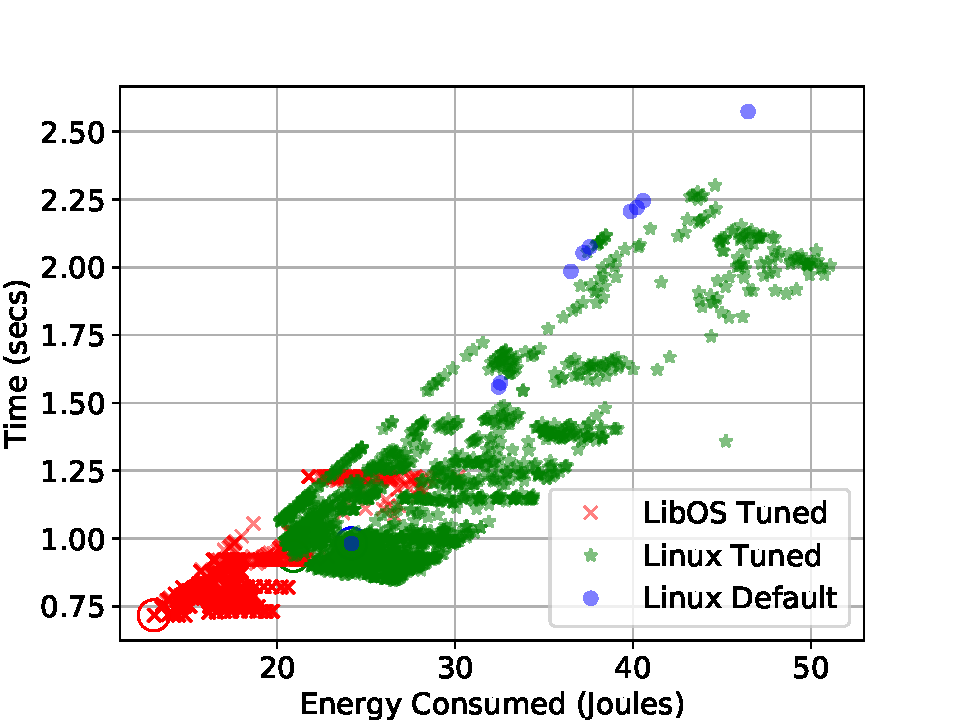
\includegraphics[width=\textwidth]{osdi_figures/netpipe_65536_overview.pdf}
        \end{subfigure}
%        \hfill
        \begin{subfigure}[b]{0.45\textwidth}  
            \centering 
            \caption[]%
            {{\small Memcached 600K QPS}} 
            \vspace*{-0.25cm}    
            \label{fig:mcdov}
            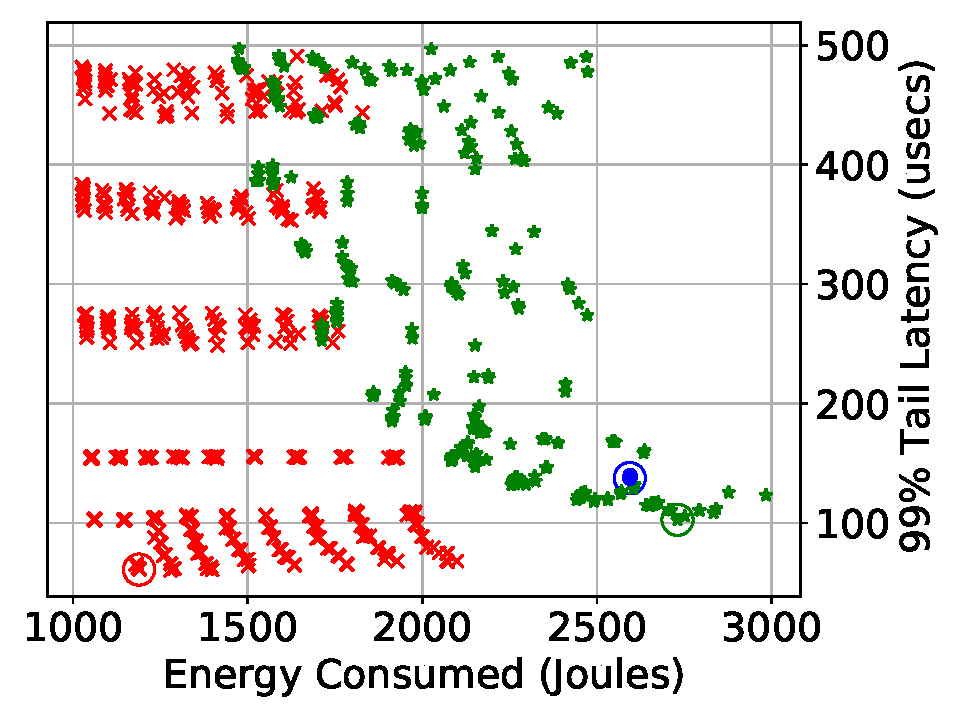
\includegraphics[width=\textwidth]{osdi_figures/mcd_600000_overview.pdf}
        \end{subfigure}
        \vskip\baselineskip
        \vspace*{-0.47cm} 
        \begin{subfigure}[b]{0.45\textwidth}   
            \centering 
            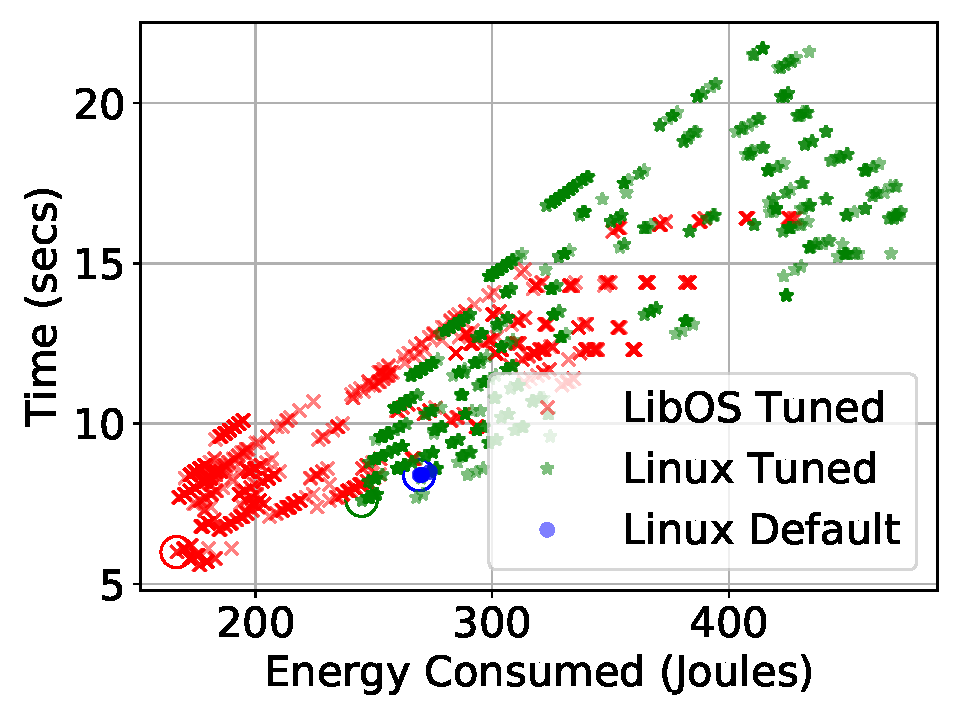
\includegraphics[width=\textwidth]{osdi_figures/nodejs_overview.pdf}
            \caption[]%
                    {{\small NodeJS 100K requests}}
                    %\hspace*{0.35cm}  
            \label{fig:nodejsov}
        \end{subfigure}
%        \hfill
        \begin{subfigure}[b]{0.45\textwidth}   
            \centering 
            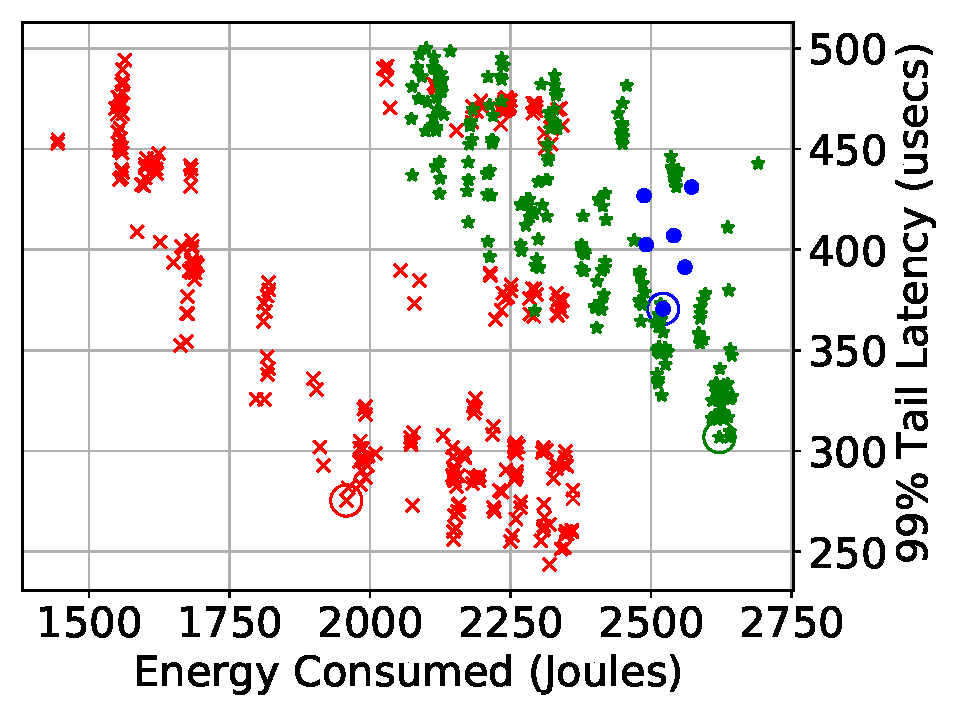
\includegraphics[width=\textwidth]{osdi_figures/mcdsilo_200000_overview.pdf}
            \caption[]%
            {{\small Memcached-silo 200K QPS}}    
            \label{fig:mcdsiloov}
        \end{subfigure}
        \caption[]
                {\small
These landscape plots portray the space of energy-performance profiles
that an OS/workload software stack can exhibit. The circle around individual points represent the min EPP values achieved in each workload.
\textit{Note that, in these plots, the origins do not start at zero
because the aim of the plots is to highlight structure within a plot
rather than to draw a comparison across plots.}
                  %Data from a run the settings associated with the 'best' EPP points are presented in~\ref{sec:data} and discussed in~\ref{sec:details}.          %Using these values we plot a timeline of the joule readings for one experimental run at the setting for Linux tuned and libOS along with data from a default Linux run of the workload.  The x-axis is the time offset from the beginning of the experiment.  For each log entry with a joule reading, we plot its value against its timestamp offset from the beginning of the run.  While the log has entries for every interrupt, we restrict sampling the joule counter to be at least 1ms apart as per the hardware manual's recommendation, as such not all log entries have an associated joule value.  To improve readability we only show a subset of the markers and use a line to connect the visible marks to the points not shown.    
        } 
        \label{fig:overview}
    \end{figure*}



%In this paper, we investigate the impact of hardware tuning on the performance and energy consumption of applications running on top of two baremetal OSes with fundamentally different design and implementation.
This study grew out of our efforts to explore a baremetal library OS for running datacenter workloads.
When configuring the library OS, we began by inheriting the default values that Linux uses on the same hardware.
However, it soon became clear that Linux's behaviour with respect to these settings was a complex mixture of dynamic and administrator controlled parameters.  
The actual impact and optimality of Linux's defaults on the energy consumption and realized application performance was not discernible though inspection and reasoning alone.
As a result, we decided to explore in detail the performance and energy use of both Linux and our library OS under a variety of hardware settings and workloads. 

We focus our study on three hardware settings - 1) Network Interface Card (NIC) Interrupt delay (ITR-delay), 2) Dynamic Voltage and Frequency Scaling (DVFS) and 3) Running Average Power Limit (RAPL) -
and four network-driven workloads (Table~\ref{table:wrkcfgs}) that span open and closed-loop dynamics with both low and high application CPU requirements. 
While open-loop latency-critical workloads tend to be common in the cloud, closed-loop workloads expose scenarios in which there is an interdependence between service performance and the offered load.
The range of closed-versus-open and high-versus-low CPU demand provides a rich ground for exposing and analyzing the behavior of the two target OSes.



%\subsection*{Summary of Findings}

We compare the performance of default Linux
running the workloads under the 11 scenarios in Table~\ref{table:wrkcfgs}
to that of {\em tuned} Linux and {\em tuned} library OS,
both configured across a wide range of static values
for the three hardware settings.   
We built infrastructure in both systems to collect detailed time series log data on every network interrupt (see Section \ref{sec:log_collect} for details).
This data includes a high-precision timestamp, Joules consumed, instructions and cycles executed, sleep states entered, last-level cache misses, and bytes received and transmitted.
The results in this paper include data from tens of thousands of experiments, each supported by detailed logs.

Figures~\ref{fig:netpipe64Kov}-~\ref{fig:mcdsiloov}
show example landscape plots that summarize many experiments
and showcase trends in the global energy-performance
exhibited by the different OS/workload pairs we explore.
Each point shows the performance-versus-energy consumed in a single experiment,
whereby performance metrics are chosen
in concert with workload requirements:
response-time for best-effort tasks
and \% tail-latency for latency-critical tasks.
The circled points in each figure
represent experiments that achieved the best energy-performance
\footnote{Note that best energy-performance is analogous to
lowest Energy Performance Product (EPP).}.
We discuss these points in depth in section \S\ref{sec:analysis}.

This paper presents a careful and comprehensive analysis of
our collected experimental data.
We structure our analysis around four questions
that we refer back to throughout the paper.
We begin by presenting these questions
and some of the insights they motivate:
%\vspace{3pt}
%\subsection{Organizing Questions}
\begin{compactdesc}
\item[Q1:] {\bf What impact does OS path length have on system-wide energy consumption?}
%Short OS path length has a direct and expected impact on energy consumption,
Short OS path length has a direct impact on energy consumption in netpipe and memcached where the OS is more prominent.
Our data(~\ref{fig:netpipe64Kov} and~\ref{fig:mcdov}) suggests short OS path lengths increase the opportunity to halt and/or slow down the processor to further reduce energy.
%(see Figures~\ref{fig:netpipe64Kov} and~\ref{fig:mcdov}).

%The number of instructions spent on OS functionality has subtle implications when it comes to energy consumption, particularly for OS-centric applications. 
%Figures~\ref{fig:netpipe64Kov} and~\ref{fig:mcdov} illustrate the energy-performance landscapes of NetPIPE and Memcached, both OS-centric workloads.
%The notable energy-performance of these workloads on our library OS leads us to posit that shortened OS path lengths must allow for greater opportunity to exploit gaps in processing, during which the processor can be halted or slowed down.

\item[Q2] {\bf What impact does low-level OS behavior have on the net efficiency when executing an application-centric software stack?}
The OS can have a surprisingly large impact (30\% improvement)
on the application cycles-per-instruction (CPI).
Figures~\ref{fig:nodejsov} and~\ref{fig:mcdsiloov}
illustrate this impact on nodejs and memcached-silo. Moreover, it appears that event-driven library OS techniques (see \S\ref{sec:OS_libos}) can both improve performance and lower energy by up to 48\% even on two application-centric workloads.

%but indirectly lead to significant improvements in the energy efficiency
%of constituent resident applications. 
%such as removing domain crossings,
%running to completion,
%and dispatching of application code from an interrupt,


%The behavior of the OS can significantly impact application cycles-per-instruction (CPI), particularly for application-centric tasks.
%Figures~\ref{fig:nodejsov} and~\ref{fig:mcdsiloov} show that, for NodeJS and Memcached-Sile, both application-centric workloads, the library OS is able to achieve energy-performance improvements larger than the best improvements possible on Linux.
%We attribute this advantage to the execution model of the library OS and assert its fidelity as an environment for energy efficient solutions.

\item[Q3] {\bf In what ways does the OS adjust during idle periods to save energy?}
We discover a hardware setting effect where a low processor frequeuncy can cause libOS to transition between interrupt and poll-driven network-bound processing in a slow-to-stay-busy manner - an optimization not explicitly built into it its software. In the two closed loop workloads, we found staying busy to finish work fast resulted in better energy and time savings. Further, another tactic is aggressively increasing network interrupt delays can induce longer idle periods and more often at the expense of SLA budgets.
%Under particular low-energy hardware configurations, the OS behavior can exhibit fascinating trends.
%For example, we see, even in a simple library OS, that the system can adopt an optimization which is not explicitly built into it, whereby the library OS seemlessly transitions between interrupt and poll-driven network-bound processing.

%Sections \S\ref{sec:OS_linux} and \S\ref{sec:OS_libos} discuss OS idle time management in Linux and our library OS and highlight a surprising behavior exhibited by the library OS under particular hardware energy configurations.

\item[Q4] {\bf What is the impact of complex OS energy management, design, and implementation on energy use?}
By disabling dynamic policies of a general purpose, we are able to both reduce energy and increase performance by adjusting settings manually. We found manual adjusting expands the trade-off space and in some cases even take advantage of hardware settings outside of dynamic policy bounds.
%Figures~\ref{fig:netpipe64Kov}-\ref{fig:mcdsiloov} give us insight on the valid ranges of energy-tuning settings that each OS can apply.
%Section \S\ref{sec:OS_linux}  outlines possible energy-tuning limitations incurred by complex OS subsystems and power management policies built into the OS.
%The dynamic policies of a general-purpose OS,
%which make complex and sophisticated decisions
%that involve integration with different parts of the system,
%may well make it more difficult to tune
%the overall system performance and efficiency
%(see \S\ref{sec:OS_linux}).
%{\em We find that there may well exist a virtuous cycle,
%where simplifying code paths and removing local policies
%enables more comprehensive and efficient global tuning,
%which will, in turn, enable further simplification and improved performance.}

%Are tuning parameters and their effectiveness a characteristic of the OS?
\end{compactdesc}

We resume this paper by
framing our study in the context of the related works in Section \ref{sec:related}.
We then discuss our target experimental setup in Section \ref{sec:exp},
including the hardware components and parameters,
application workloads,
and OSes used.
We continue on to present an overview of our observations in Section \ref{sec:resoverview} followed by a detailed analysis in Section \ref{sec:analysis}.



